\documentclass{bbawslides}

\usepackage{ifthen}

\usepackage[a4paper]{hyperref}
\rotateheaderstrue	%%-- otherwise seminar does strange things
\usepackage{url}

\usepackage[ngerman]{babel}
\usepackage[babel]{csquotes}
\usepackage[autoplay]{animate}
\usepackage{graphicx}


\begin{document}
\providecommand{\Title}{}


\begin{bbawtitle}[(Open-Source-)OCR-Workflows]
  \vspace*{3em}%
  Kay-Michael Würzner\\[-.25em]%
  \textcolor{urlColor}{\texttt{{\small wuerzner@bbaw.de}}}
  \\[3em]
  {\footnotesize{%
    DH-Kolloquium an der Berlin-Brandenburgischen Akademie der Wissenschaften\\%
    4. August 2017\\%
  }}
\end{bbawtitle}
\slideStyleFrame

\renewcommand{\footerText}{\tiny 4. August 2017, DH-Kolloquium, BBAW}

%----------------------------------------------------------------------------------------------
% Outline
%----------------------------------------------------------------------------------------------
\begin{bbawslide}{Übersicht}
  \vspace*{7mm}%
  \centerslidestrue%
  \begin{itemize}
  \item Was ist OCR?
  \item Wozu braucht man OCR?
  \item Komponenten eines OCR-Workflows
  \item Modelltraining
  \item Optimierungsoptionen
  \item Warum braucht man OCR (i.e. DH-Perspektiven)?
  \item OCR-D
  \end{itemize}
\end{bbawslide}

\begin{bbawpart}{\Large\bf Was ist OCR?}
\end{bbawpart}

\begin{bbawslide}{Was ist OCR?}
  \vspace*{7mm}%
  \centerslidestrue%
  \begin{tabular}{lc}
    \begin{minipage}{0.6\textwidth}
      \begin{itemize}
        \item \textbf{O}ptical \textbf{C}haracter \textbf{R}ecognition: Automatische Erfassung von Text in Bildern
        \item ursprünglich begrenzt auf Zeichenerkennung
        \item heute häufig Synonym für den gesamten Texterfassungsprozess
        \begin{itemize}
          \item Bildvorverarbeitung
          \item Layoutanalyse (OLR)
          \item Zeilenerkennung
          \item \ldots
        \end{itemize}
      \end{itemize}
    \end{minipage}
    &
    \begin{minipage}{0.4\textwidth}
      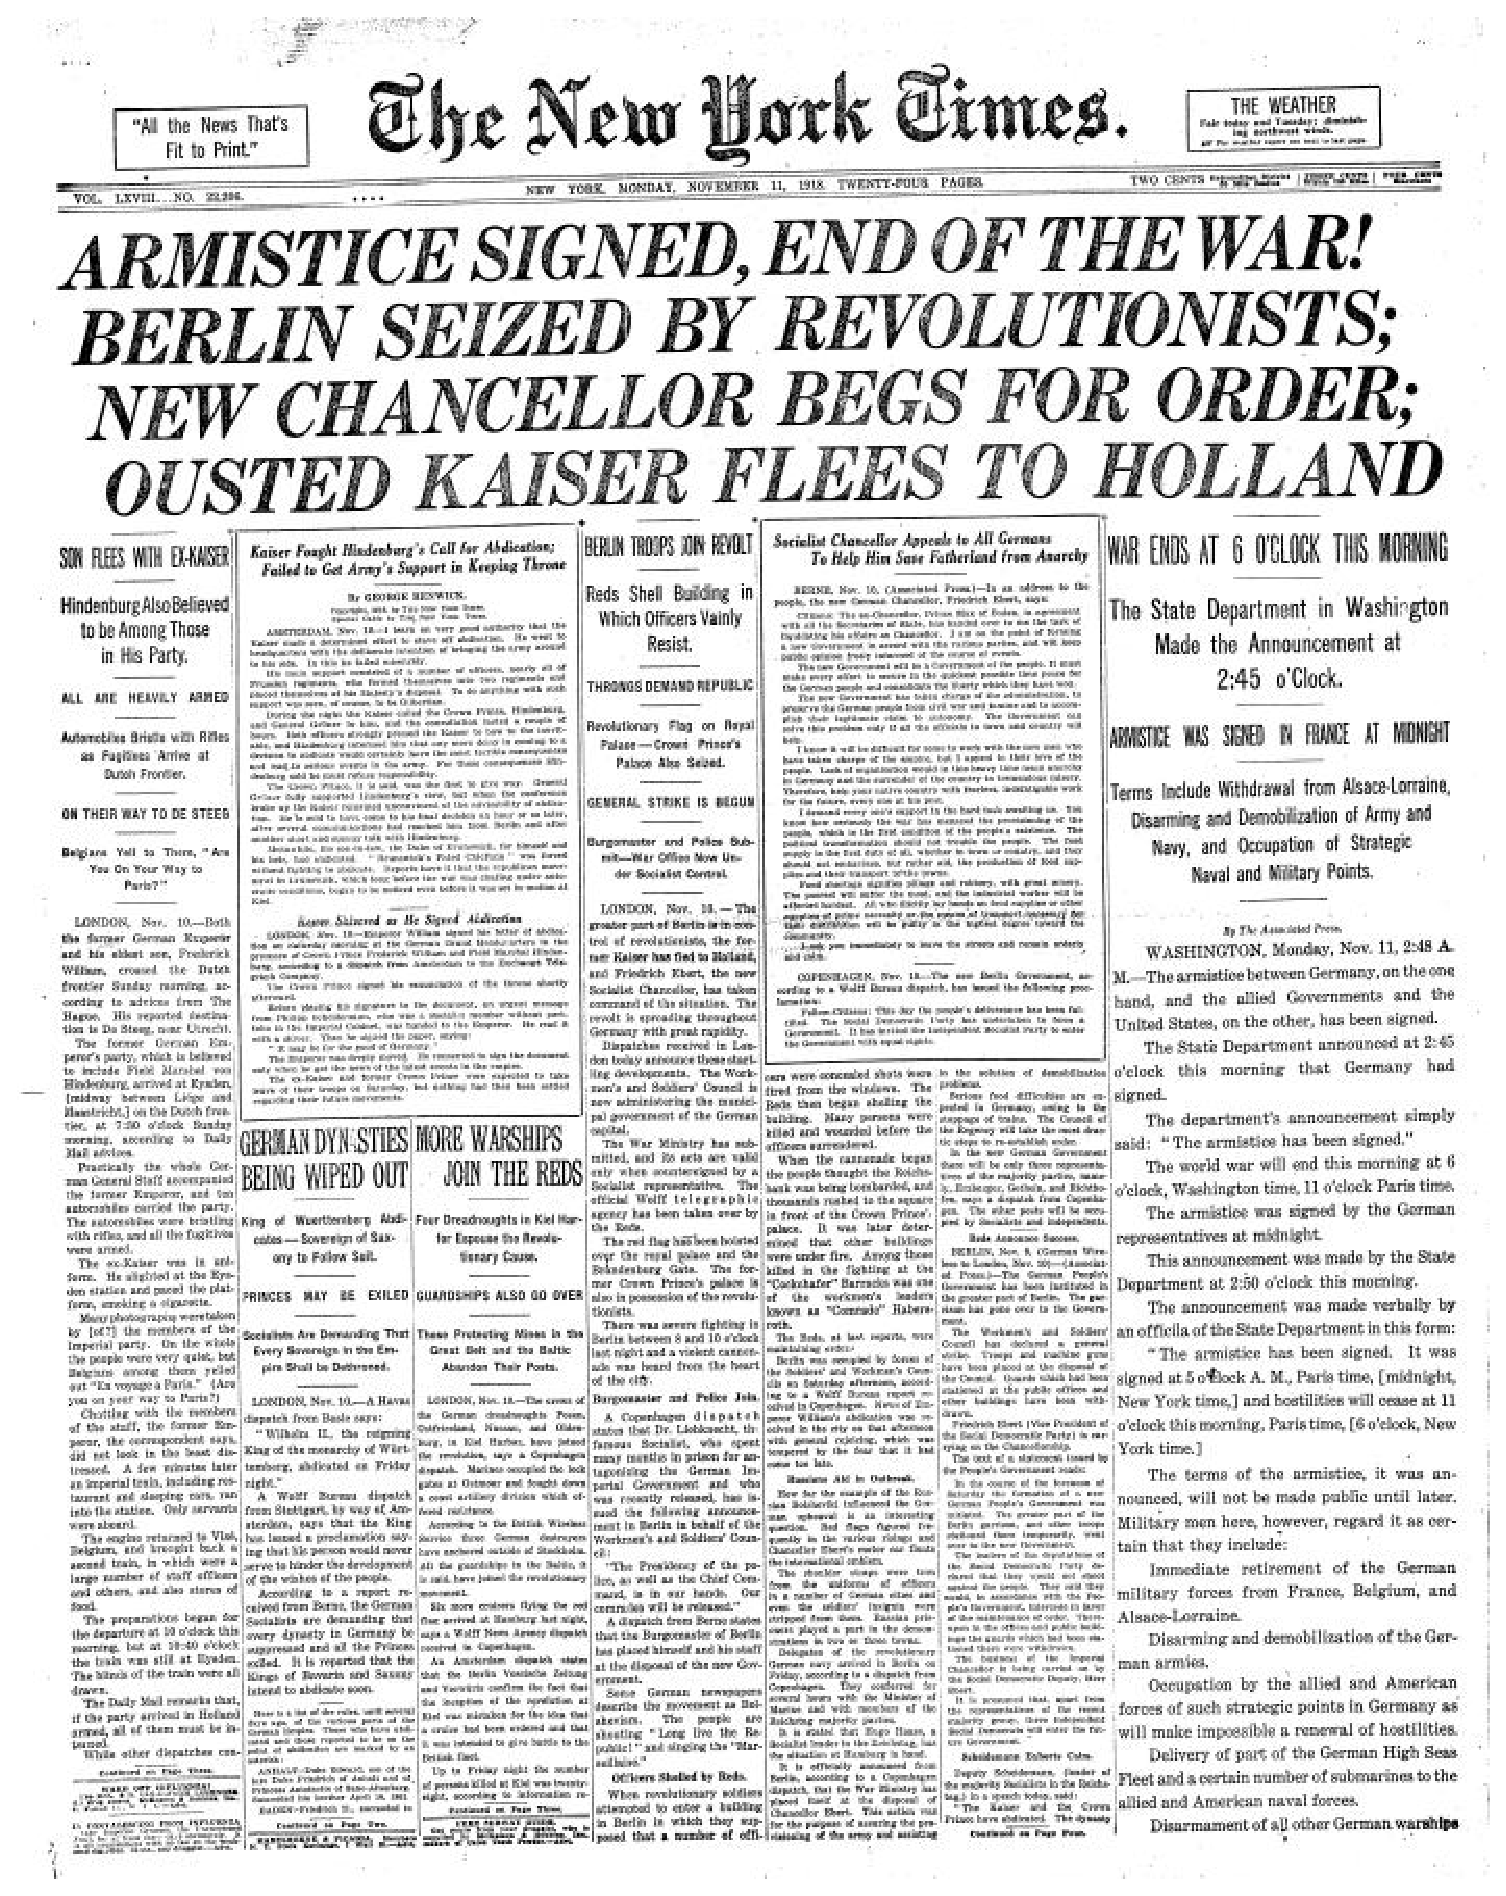
\epsfig{file=figures/times.eps,width=\textwidth}
    \end{minipage}
  \end{tabular}
\end{bbawslide}

\begin{bbawslide}{Zeichenorientierte Ansätze}
  \vspace*{7mm}%
  \hspace*{-2em}%
  \centerslidestrue%
  \begin{tabular}{lc}
    \begin{minipage}{0.68\textwidth}
      \begin{mitemize}
      \item Erkennung erfolgt \emph{glyphenweise}
        \begin{description}\small
          \item[Pattern matching:] Vergleich der Zeichenbilder zu in einem \enquote{Setzkasten} gespeicherten Glyphen \textbf{Pixel für Pixel}
          \item[Feature extraction:] Zerlegung der Glyphen in vordefinierte, bedeutungstragende \textbf{Eigenschaften}
          wie \emph{Einfärbung, Kurven, Linien} etc. und Vergleich zu Trainingsmaterialien
        \end{description}
      \item Kombination beider Ansätze möglich
      \item Zerlegung der Seite in \emph{Zeilen} und \emph{Zeichen} notwendig
      \item Open-Source Software \texttt{Tesseract 3} \hlcite{Smith 2007}
        \begin{mitemize}\small
          \item Einsatz verschiedener Lexika für frequente Wörter, Sonderzeichen und
        häufige Fehler zur Verbesserung der Erkennung
        \end{mitemize}
      \end{mitemize}
    \end{minipage}
    &
    \begin{minipage}{0.38\textwidth}
      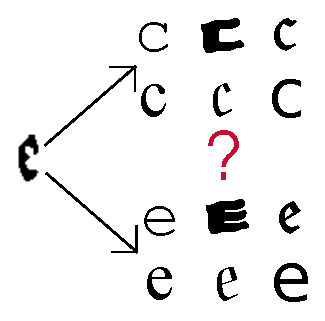
\epsfig{file=figures/char.eps,width=\textwidth}
    \end{minipage}
  \end{tabular}
\end{bbawslide}

\begin{bbawslide}{Sequenzorientierte Ansätze}
  \vspace*{7mm}%
  \centerslidestrue%
  \begin{minipage}{1.05\textwidth}
    \begin{itemize}
      \item Erkennung erfolgt \emph{zeilenweise}
        \begin{description}\small
          \item[Scaling:] Einheitliche Höhe für alle Zeilen
          \item[Feature extraction:] Grid mit festgelegter Anzahl (horizontaler) Zeilen und variabler Anzahl
                                     (vertikaler) Spalten: Zeilen als Sequenzen binärwertiger Vektoren fixer Länge
        \end{description}
    \end{itemize}
  \end{minipage}
  \begin{center}
    
\epsfig{file=figures/grid.eps,width=1.05\textwidth}
  \end{center}
  \begin{minipage}{1.05\textwidth}
    \begin{itemize}
      \item Kontextsensitive (i.e.~ über \emph{Übergangswahrscheinlichkeiten} der Vektoren) Erkennung
      \item Zerlegung der Seite in \emph{Zeilen} notwendig
      \item Vorgehen (normalerweise) \emph{robuster} gegenüber Varianz durch Artefakte als zeichenorientierte Ansätze
      \item Open-Source Software \texttt{OCRopus} \hlcite{Breuel 2008}
      \begin{mitemize}\small
        \item Einsatz \emph{neuronaler Netzwerke} für die Sequenzklassifikation
      \end{mitemize}
    \end{itemize}
  \end{minipage}
\end{bbawslide}

\begin{bbawpart}{\Large\bf Wozu braucht man OCR?}
\end{bbawpart}

\renewcommand{\footerText}{\tiny 4. August 2017, DH-Kolloquium, BBAW\hspace{4cm} Image by Achim Raschka, CC BY-SA 3.0}

\begin{bbawslide}{Wozu braucht man OCR?}
  \vspace*{1mm}%
  \centerslidesfalse%
  \begin{tabular}{cc}
    \raisebox{-\height}{\parbox{7cm}{%
      \begin{itemize}
        \item typische Anwendungen:
        \begin{itemize}\small
          \item Nummernschilderkennung (\emph{Automatic number plate recognition})
        \end{itemize}
      \end{itemize}
    }}
    &
    \raisebox{-\height}{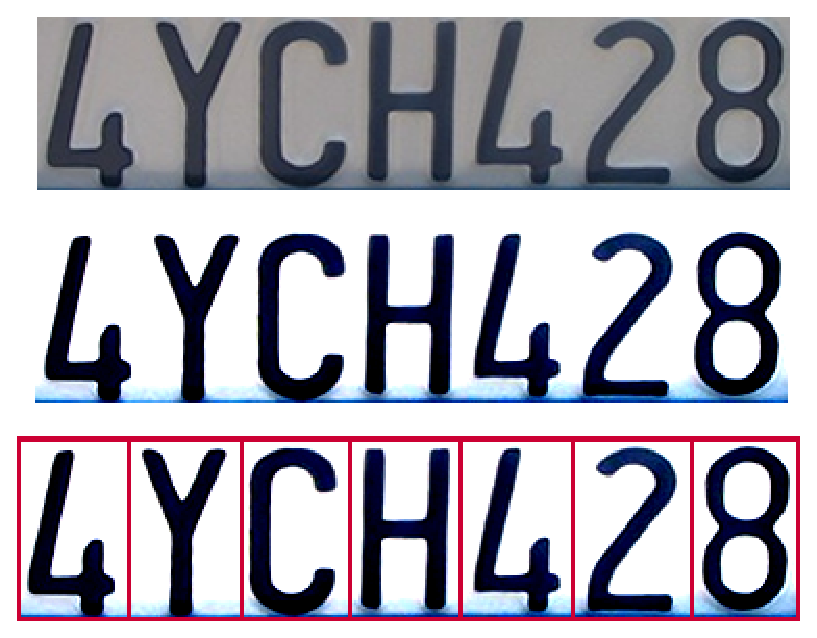
\epsfig{file=figures/ANPR.eps,width=0.4\textwidth}}%
  \end{tabular}
\end{bbawslide}

\renewcommand{\footerText}{\tiny 4. August 2017, DH-Kolloquium, BBAW\hspace{4cm} Image by JD, CC BY-SA 2.0}

\begin{bbawslide}{Wozu braucht man OCR?}
  \vspace*{1mm}%
  \centerslidesfalse%
  \begin{tabular}{cc}
    \raisebox{-\height}{\parbox{7cm}{%
      \begin{itemize}
        \item typische Anwendungen:
        \begin{itemize}\small
          \item Nummernschilderkennung (\emph{Automatic number plate recognition})
          \item Captcha-Umgehung (\emph{Completely Automated Public Turing test to tell Computers and Humans Apart})
        \end{itemize}
      \end{itemize}
    }}
    &
    \raisebox{-\height}{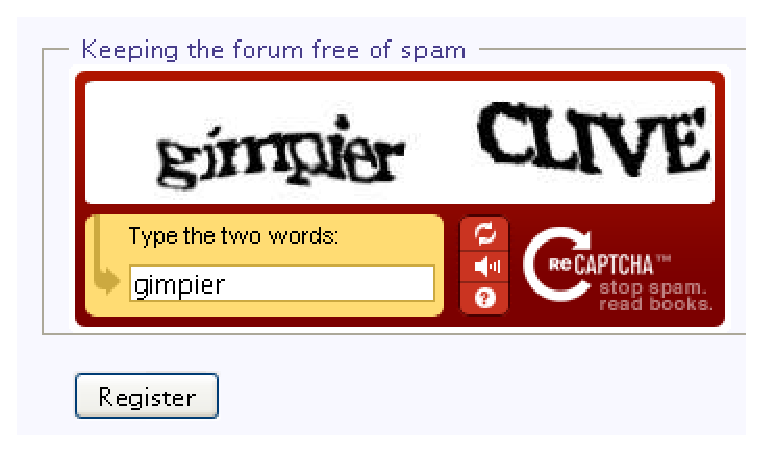
\epsfig{file=figures/Captcha.eps,width=0.4\textwidth}}%
  \end{tabular}
\end{bbawslide}

\renewcommand{\footerText}{\tiny 4. August 2017, DH-Kolloquium, BBAW\hspace{4cm} Image by Eluminary, CC BY-SA 4.0}

\begin{bbawslide}{Wozu braucht man OCR?}
  \vspace*{1mm}%
  \centerslidesfalse%
  \begin{tabular}{cc}
    \raisebox{-\height}{\parbox{7cm}{%
      \begin{itemize}
        \item typische Anwendungen:
        \begin{itemize}\small
          \item Nummernschilderkennung (\emph{Automatic number plate recognition})
          \item Captcha-Umgehung (\emph{Completely Automated Public Turing test to tell Computers and Humans Apart})
          \item Schlüsselinformationsextraktion (\emph{Document's key information extraction})
        \end{itemize}
      \end{itemize}
    }}
    &
    \raisebox{-\height}{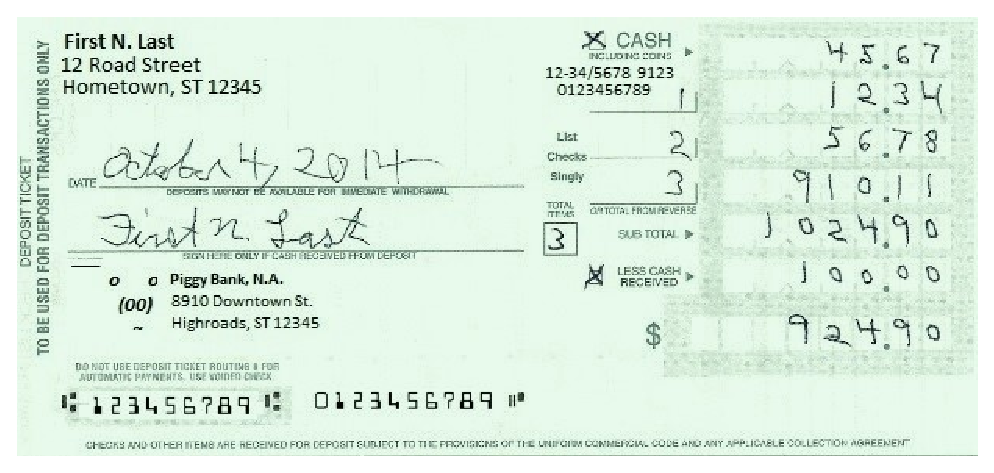
\epsfig{file=figures/deposit.eps,width=0.4\textwidth}}%
  \end{tabular}
\end{bbawslide}

\renewcommand{\footerText}{\tiny 4. August 2017, DH-Kolloquium, BBAW}

\begin{bbawslide}{Wozu braucht man OCR?}
  \vspace*{1mm}%
  \centerslidesfalse%
  \begin{tabular}{cc}
    \raisebox{-\height}{\parbox{7cm}{%
      \begin{itemize}
        \item typische Anwendungen:
        \begin{itemize}\small
          \item Nummernschilderkennung (\emph{Automatic number plate recognition})
          \item Captcha-Umgehung (\emph{Completely Automated Public Turing test to tell Computers and Humans Apart})
          \item Schlüsselinformationsextraktion (\emph{Document's key information extraction})
          \item Handschrifterkennung (\emph{Handwritten text recognition})
        \end{itemize}
      \end{itemize}
    }}
    &
    \raisebox{-\height}{\epsfig{file=figures/transkribus.eps,width=0.4\textwidth}}%
  \end{tabular}
\end{bbawslide}

\renewcommand{\footerText}{\tiny 4. August 2017, DH-Kolloquium, BBAW\hspace{4cm} Images by Uwe Springmann, CC BY-SA 4.0}

\begin{bbawslide}{Wozu braucht man OCR?}
  \vspace*{1mm}%
  \centerslidesfalse%
  \begin{tabular}{cc}
    \raisebox{-\height}{\parbox{7cm}{%
      \begin{itemize}
        \item typische Anwendungen:
        \begin{itemize}\small
          \item Nummernschilderkennung (\emph{Automatic number plate recognition})
          \item Captcha-Umgehung (\emph{Completely Automated Public Turing test to tell Computers and Humans Apart})
          \item Schlüsselinformationsextraktion (\emph{Document's key information extraction})
          \item Handschrifterkennung (\emph{Handwritten text recognition})
          \item \textbf{Volltextdigitalisierung}
        \end{itemize}
      \end{itemize}
    }}
    &
    \raisebox{-\height}{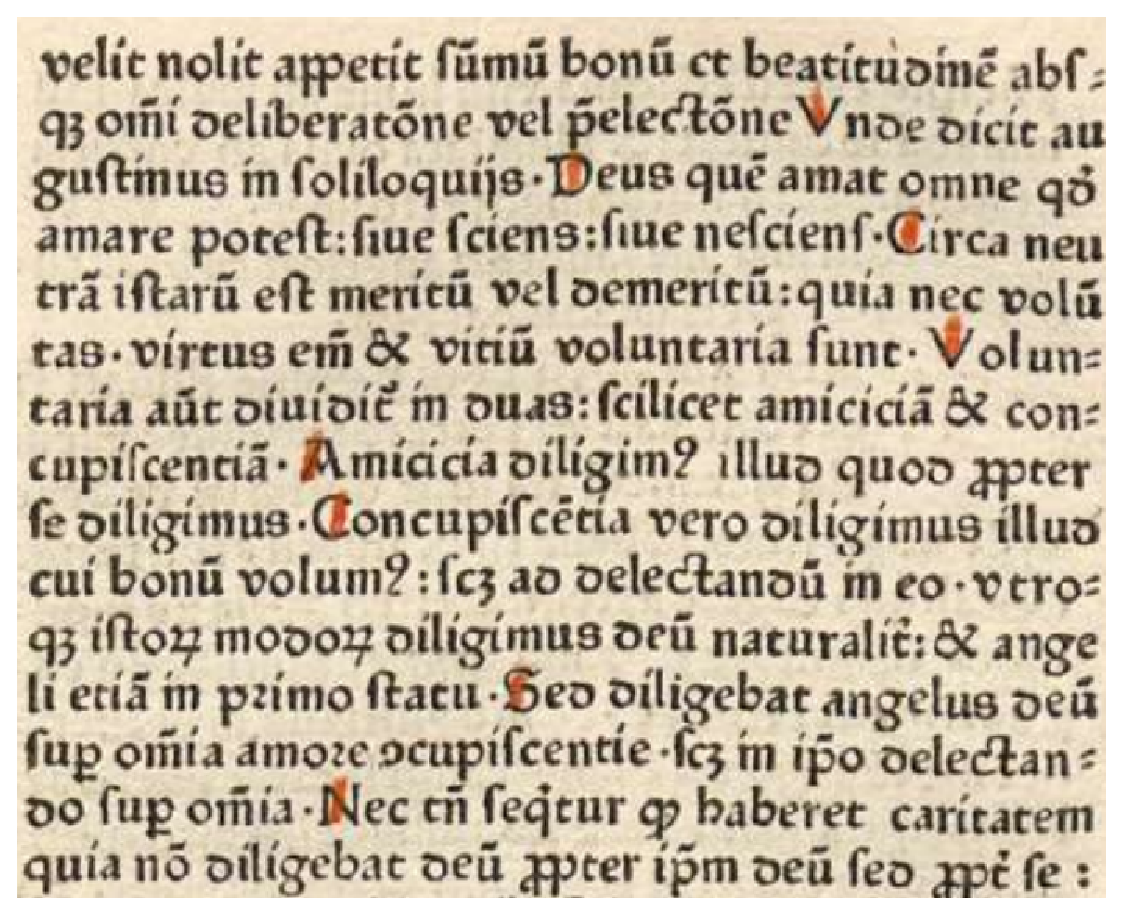
\epsfig{file=figures/beauvais_0.eps,width=0.4\textwidth}}%
  \end{tabular}
\end{bbawslide}

\begin{bbawslide}{Wozu braucht man OCR?}
  \vspace*{1mm}%
  \centerslidesfalse%
  \begin{tabular}{cc}
    \raisebox{-\height}{\parbox{7cm}{%
      \begin{itemize}
        \item typische Anwendungen:
        \begin{itemize}\small
          \item Nummernschilderkennung (\emph{Automatic number plate recognition})
          \item Captcha-Umgehung (\emph{Completely Automated Public Turing test to tell Computers and Humans Apart})
          \item Schlüsselinformationsextraktion (\emph{Document's key information extraction})
          \item Handschrifterkennung (\emph{Handwritten text recognition})
          \item \textbf{Volltextdigitalisierung}
        \end{itemize}
      \end{itemize}
    }}
    &
    \raisebox{-\height}{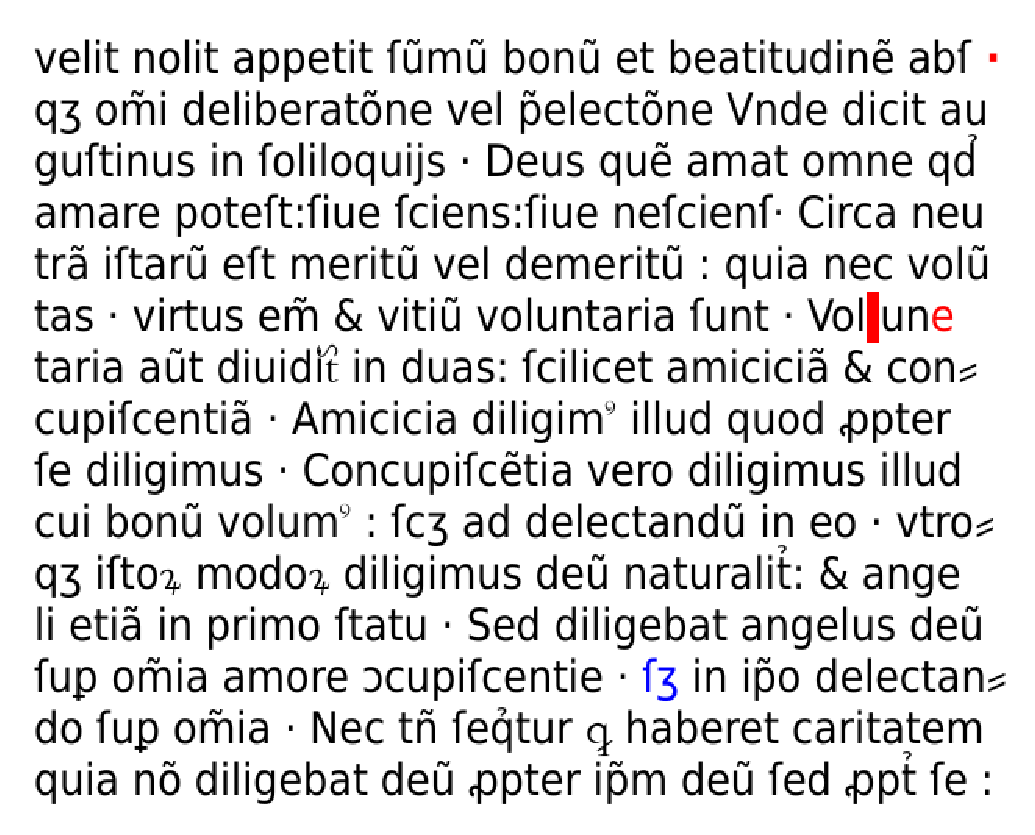
\epsfig{file=figures/beauvais_1.eps,width=0.4\textwidth}}%
  \end{tabular}
\end{bbawslide}

\renewcommand{\footerText}{\tiny 4. August 2017, DH-Kolloquium, BBAW}

\begin{bbawpart}{\Large\bf Komponenten eines OCR-Workflows}
\end{bbawpart}

\begin{bbawslide}{Komponenten eines OCR-Workflows}
  \vspace*{2mm}%
  \centerslidestrue%
  \begin{tabular}{cc}
    \phantom{\raisebox{-3\height}{\parbox{7cm}{%
      \begin{enumerate}
        \item Bildvorverarbeitung
        \item Layoutanalyse
        \item Texterkennung
      \end{enumerate}
    }}}
    &
    \raisebox{-\height}{\epsfig{file=figures/grenzboten_raw.eps,width=0.4\textwidth}}%
  \end{tabular}
\end{bbawslide}

\begin{bbawslide}{Komponenten eines OCR-Workflows}
  \vspace*{2mm}%
  \centerslidestrue%
  \begin{tabular}{cc}
    \raisebox{-3\height}{\parbox{7cm}{%
      \begin{enumerate}
        \item Bildvorverarbeitung
        \item
        \item
      \end{enumerate}
    }}
    &
    \raisebox{-\height}{\epsfig{file=figures/grenzboten_raw.eps,width=0.4\textwidth}}%
  \end{tabular}
\end{bbawslide}

\begin{bbawslide}{Komponenten eines OCR-Workflows}
  \vspace*{2mm}%
  \centerslidestrue%
  \begin{tabular}{cc}
    \raisebox{-3\height}{\parbox{7cm}{%
      \begin{enumerate}
        \item Bildvorverarbeitung
        \item
        \item
      \end{enumerate}
    }}
    &
    \raisebox{-\height}{\epsfig{file=figures/grenzboten_opt.eps,width=0.4\textwidth}}%
  \end{tabular}
\end{bbawslide}

\begin{bbawslide}{Komponenten eines OCR-Workflows}
  \vspace*{2mm}%
  \centerslidestrue%
  \begin{tabular}{cc}
    \raisebox{-3\height}{\parbox{7cm}{%
      \begin{enumerate}
        \item Bildvorverarbeitung
        \item Layoutanalyse
        \item
      \end{enumerate}
    }}
    &
    \raisebox{-\height}{\epsfig{file=figures/grenzboten_opt.eps,width=0.4\textwidth}}%
  \end{tabular}
\end{bbawslide}

\begin{bbawslide}{Komponenten eines OCR-Workflows}
  \vspace*{2mm}%
  \centerslidestrue%
  \begin{tabular}{cc}
    \raisebox{-3\height}{\parbox{7cm}{%
      \begin{enumerate}
        \item Bildvorverarbeitung
        \item Layoutanalyse
        \item
      \end{enumerate}
    }}
    &
    \raisebox{-\height}{\epsfig{file=figures/grenzboten_struct.eps,width=0.4\textwidth}}%
  \end{tabular}
\end{bbawslide}

\begin{bbawslide}{Komponenten eines OCR-Workflows}
  \vspace*{2mm}%
  \centerslidestrue%
  \begin{tabular}{cc}
    \raisebox{-3.001\height}{\parbox{7cm}{%
      \begin{enumerate}
        \item Bildvorverarbeitung
        \item Layoutanalyse
        \item Texterkennung
      \end{enumerate}
    }}
    &
    \raisebox{-\height}{\epsfig{file=figures/grenzboten_struct.eps,width=0.4\textwidth}}%
  \end{tabular}
\end{bbawslide}

\begin{bbawslide}{Komponenten eines OCR-Workflows}
  \vspace*{2mm}%
  \centerslidestrue%
  \begin{tabular}{cc}
    \raisebox{-3.001\height}{\parbox{7cm}{%
      \begin{enumerate}
        \item Bildvorverarbeitung
        \item Layoutanalyse
        \item Texterkennung
      \end{enumerate}
    }}
    &
    \raisebox{-\height}{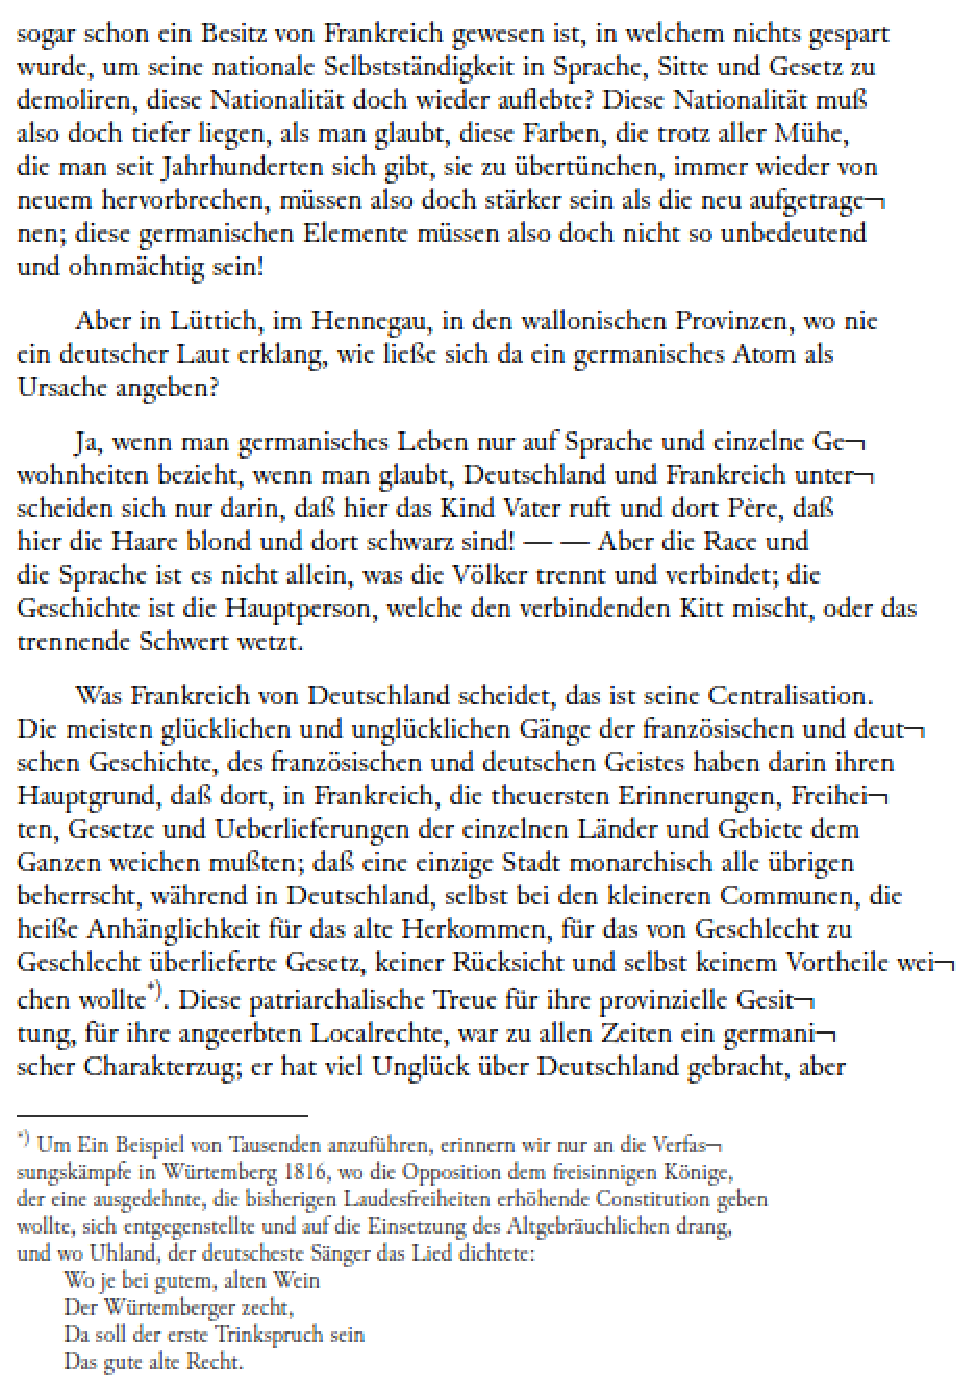
\epsfig{file=figures/grenzboten_text.eps,width=0.4\textwidth}}%
  \end{tabular}
\end{bbawslide}

\begin{bbawslide}{Komponenten eines OCR-Workflows: Bildvorverarbeitung}
  \vspace*{7mm}%
  \centerslidestrue%
  \begin{itemize}
    \item Prozesse zur bestmöglichen Vorbereitung der Digitalisate für OLR und OCR
    \begin{itemize}\small
      \item \textbf{Cropping:} Beschneidung des Digitalisats auf den Druckbereich
      \item \textbf{Deskewing:} Rotation des Digitalisats zur Begradigung von Schrägstellungen
      \item \textbf{Despeckling:} Entfernung von Bildartefakten (Verschmutzungen, sichtbare Papiermaserung etc.)
      \item \textbf{Binarization:} Binäre Kodierung der Pixel (bedruckte Bereiche schwarz, nicht-bedruckte Bereiche weiß)
      \item \textbf{Dewarping:} Begradigung von Wellen auf Zeilenebene
    \end{itemize}
    \item starker Einfluss auf die Erkennungsqualität
  \end{itemize}
\end{bbawslide}

\begin{bbawslide}{Komponenten eines OCR-Workflows: Cropping}
  \vspace*{7mm}%
  \centerslidestrue%
  \begin{itemize}
    \item
  \end{itemize}
\end{bbawslide}

\begin{bbawslide}{Komponenten eines OCR-Workflows: Deskewing}
  \vspace*{7mm}%
  \centerslidestrue%
  \begin{itemize}
    \item
  \end{itemize}
\end{bbawslide}

\begin{bbawslide}{Komponenten eines OCR-Workflows: Despeckling}
  \vspace*{7mm}%
  \centerslidestrue%
  \begin{itemize}
    \item
  \end{itemize}
\end{bbawslide}

\begin{bbawslide}{Komponenten eines OCR-Workflows: Binarization}
  \vspace*{7mm}%
  \centerslidestrue%
  \begin{itemize}
    \item
  \end{itemize}
\end{bbawslide}

\begin{bbawslide}{Komponenten eines OCR-Workflows: Dewarping}
  \vspace*{7mm}%
  \centerslidestrue%
  \begin{itemize}
    \item
  \end{itemize}
\end{bbawslide}

\begin{bbawpart}{\Large\bf Modelltraining}
\end{bbawpart}

\begin{bbawslide}{Modelltraining}
  \vspace*{7mm}%
  \centerslidestrue%
  \begin{itemize}
    \item
  \end{itemize}
\end{bbawslide}

\begin{bbawpart}{\Large\bf Optimierungsoptionen}
\end{bbawpart}

\begin{bbawslide}{Optimierungsoptionen}
  \vspace*{7mm}%
  \centerslidestrue%
  \begin{itemize}
    \item
  \end{itemize}
\end{bbawslide}

\begin{bbawpart}{\Large\bf Warum braucht man OCR?}
\end{bbawpart}

\begin{bbawslide}{Warum braucht man OCR?}
  \vspace*{7mm}%
  \centerslidestrue%
  \begin{itemize}
    \item
  \end{itemize}
\end{bbawslide}

\begin{bbawpart}{\Large\bf OCR-D}
\end{bbawpart}

\begin{bbawslide}{OCR-D}
  \vspace*{7mm}%
  \centerslidestrue%
  \begin{itemize}
    \item
  \end{itemize}
\end{bbawslide}

\end{document}

%
% modelines
%

%%% Local Variables:
%%% mode: LaTeX
%%% coding: utf-8
%%% tab-width: 2
%%% indent-tabs-mode: nil
%%% End:

% vim: set ts=2 sw=2 expandtab :
